\documentclass{article}

% Recommended, but optional, packages for figures and better typesetting:
\usepackage{microtype}
\usepackage{graphicx}
\usepackage{subfigure}
\usepackage{booktabs} % for professional tables

% hyperref makes hyperlinks in the resulting PDF.
% If your build breaks (sometimes temporarily if a hyperlink spans a page)
% please comment out the following usepackage line and replace
% \usepackage{icml2021} with \usepackage[nohyperref]{icml2021} above.
\usepackage{hyperref}

% Attempt to make hyperref and algorithmic work together better:
\newcommand{\theHalgorithm}{\arabic{algorithm}}

% Use the following line for the initial blind version submitted for review:
%\usepackage{icml2021}

% If accepted, instead use the following line for the camera-ready submission:
\usepackage[accepted]{icml2021}

% The \icmltitle you define below is probably too long as a header.
% Therefore, a short form for the running title is supplied here:
\icmltitlerunning{TimelyWimely: Classifying Timely And Timeless Questions}

\begin{document}

\twocolumn[
	\icmltitle{Wibbly Wobbly Timely Wimely Questions: \\Classifying Timely And Timeless Questions}

	% It is OKAY to include author information, even for blind
	% submissions: the style file will automatically remove it for you
	% unless you've provided the [accepted] option to the icml2021
	% package.

	% List of affiliations: The first argument should be a (short)
	% identifier you will use later to specify author affiliations
	% Academic affiliations should list Department, University, City, Region, Country
	% Industry affiliations should list Company, City, Region, Country

	% You can specify symbols, otherwise they are numbered in order.
	% Ideally, you should not use this facility. Affiliations will be numbered
	% in order of appearance and this is the preferred way.
	\icmlsetsymbol{equal}{*}

	\begin{icmlauthorlist}
		\icmlauthor{Vatsal Agarwal}{umd}
		\icmlauthor{Pauline Comising}{umd}
		\icmlauthor{Harish Kumar}{umd}
		\icmlauthor{Madhava Paliyam}{umd}
		\icmlauthor{Nikhil Pateel}{umd}
	\end{icmlauthorlist}

	\icmlaffiliation{umd}{Department of Computer Science, University of Maryland, Maryland, USA}

	\icmlcorrespondingauthor{Nikhil Pateel}{\url{github.com/npateel/timelywimely}}
	% You may provide any keywords that you
	% find helpful for describing your paper; these are used to populate
	% the "keywords" metadata in the PDF but will not be shown in the document
	\icmlkeywords{Machine Learning, ICML}

	\vskip 0.3in]

% this must go after the closing bracket ] following \twocolumn[ ...

% This command actually creates the footnote in the first column
% listing the affiliations and the copyright notice.
% The command takes one argument, which is text to display at the start of the footnote.
% The \icmlEqualContribution command is standard text for equal contribution.
% Remove it (just {}) if you do not need this facility.

%\printAffiliationsAndNotice{}  % leave blank if no need to mention equal contribution
%\printAffiliationsAndNotice{\icmlEqualContribution} % otherwise use the standard text.

\begin{abstract}
	Classifying timely and timeless questions can be a useful task for natural
	language processing. We present a method for determining if a question is
	timely or timeless using a pretrained BERT model and the Google NQ dataset.
	Past revisions of the source Wikipedia page are retrieved and the answers are
	compared to see how they change over time. We show that we can find timely
	questions with greater than chance probability and timeless questions with
	high accuracy using our method.

\end{abstract}

\section{Problem Overview}
\label{overview}
Question answering (QA) is a fundamental task in natural language processing.
The objectives are to understand questions posed in natural language and
retrieve relevant information within a database or text to answer them. The
answers to some questions remain unchanged and static regardless of the time
they are asked. We will refer to these questions as timeless questions. As
examples, the answers to the questions “When was the Magna Carta signed” and
“Who was the first person to walk on the moon” do not change over time. On the
other hand, some questions will have different answers based on when they are
asked, and we will refer to these as timely questions. To illustrate, the answer
to “Who won the world cup” will change every four years, and the answer to “How
many farms are there in Alaska” will vary depending on how many Alaskan farms
exist at the asking time.

The purpose of our project is to build a pipeline that determines the
“timeliness” of questions, as understanding whether a question is timely or
timeless could be useful for accurate question answering. When an individual
asks a timely question, they would expect the system to return the most recent
answer. Detecting timeliness in queries is a nifty skill for voice assistant
software and chatbots; if a question is understood to be timely, updated answers
could be routinely checked to provide accurate results for possible future
queries.


\subsection{Related Work}

There has been extensive work examining methods to improve temporal reasoning in
natural language processing tasks such as question-answering. The 2002 TERQAS
workshops spurred initial work in this area and aimed to answer temporally-based
questions about events and entities in articles and lead to the development of
TimeML, a set of rules for encoding temporal information in documents
\cite{radev2002using}. \cite{breck2000another} was one of the first to build a
QA system which incorporated temporal information. \cite{saquete2009enhancing}
explored more complex strategies to incorporate temporal information.
Specifically, they proposed a method to first identify temporal questions and
decompose them into simpler questions. They then obtain answers to this set of
questions, and then recombine them following the original temporal relationships
to generate the complete answer. Recently, the TEQUILA method was described by
\cite{jia2018tequila} as an extension of \cite{saquete2009enhancing}. Thus, our
work focuses on improving the first task of better identifying temporal
questions.

\section{Methodology}
\label{methodology}


\subsection{Dataset}
\label{dataset}
We used Google’s Natural Questions (NQ) dataset \cite{nqdataset}. The dataset
has been used for open-domain question answering research, and is “the first
large publicly available dataset to pair real user queries with high quality
annotations of answers in documents”. It consists of 307,373 anonymized natural
questions asked via the Google search engine, and each question is paired with
the full HTML markup of a Wikipedia page. Human annotators have marked the
location of long and short answers to each question. A model that is trained on
the NQ dataset is required to read the full Wikipedia article, and locate the
answers. From our analysis, we estimate that less than 10\% of the questions
were timely questions.

SQuAD (Stanford Question Answering Dataset) 2.0 \cite{squaddataset} is a similar
dataset that we explored. However, it has some key differences; questions in
SQuAD have been artificially generated (unlike the real user queries of NQ), and
each question is paired with a text paragraph from a Wikipedia page (whereas NQ
provides the full page text).


\subsection{String Comparison Metrics}
\label{string methods}


\subsubsection{Levenshtein Distance}
\label{fuzzy}

We use a minimum string edit distance (otherwise known as the Levenshtein
Distance) to measure the similarity between two answers. Since this metric does
not rely on tokenization, it works well with smaller strings. The lack of word
boundaries for Levenshtein distance can also be a major issue. Words like
“kitten” and “smitten” will have a very low edit distance even though they are
linguistically very different. When combined with a tokenizer, one can sort
tokens alphabetically and then compute the Levenshtein distance to get a metric
that respects word boundaries slightly more. However, the underlying metric will
still disregard the differences in tokens. It is for this reason that we also
used a BLEU score.


\subsubsection{BLEU}
\label{bleumetric}


BLEU (BiLingual Evaluation Understudy) \cite{bleu}, our other answer difference
metric, is a measurement of overlap between one or multiple reference
sentence(s) and a candidate sentence. BLEU defines overlap as the percentage of
candidate sentence N-grams that are present in a reference sentence. When there
are multiple reference sentences, the highest score is returned. We calculated
this metric using the NLTK \cite{nltk} package for BLEU scores, specifically
utilizing the {\tt sentence\_bleu} function. The smallest unit in each function
argument is a 1-gram, often a word.


\subsection{Pipeline}
\label{pipeline}

\subsubsection{Answer Prediction}
Retrieving answers for all revisions of a single question worked as follows.
First, for each sample in a 20,000 question subset of the NQ train dataset, the
question text, question HTML, Wikipedia article link, and all short answers were
retrieved. We obtained the past revisions of the Wikipedia article for 2008,
2010, 2012, 2014, 2016, 2018, and current day by using the Wikimedia API. We
chose this time period because we felt this represented a long enough time-span
such that Wikipedia would have accurate information on most of the questions.
The HTML was parsed using the Beautiful Soup library and the first 25 paragraphs
of the article were extracted and fed to BERT along with the question.

The BERT-SQuAD model is a transformer model trained on the SQuAD dataset. BERT
is a bidirectional transformer and has been proven to be successful at many
natural language processing tasks such as machine translation and question
answering \cite{bert}. We chose to use an implementation by \cite{bertsquad}
which we believed would be successful with the NQ dataset since the two are
similar in the type of contextual information and questions that are available.
By feeding each year’s Wikipedia article revision and the question text to the
model, we acquire an answer for each year.

\subsubsection{Answer Filtering}
After getting an answer for each year, we hypothesized that a timely question
would have answers that change year to year, while a timeless question would
have similar answers no matter which year was used as the context. However,
before we could identify changes with the answers, we had to account for errors
with the model’s ability to answer questions. First, we removed any questions in
which any of the answers returned a page that did not exist, or was redirected.
Although a page that did not exist could indicate a timely question, we decided
to remove those in case there was a problem with the Wikipedia link or the
model. \begin{figure*}[ht]
	\begin{center}
		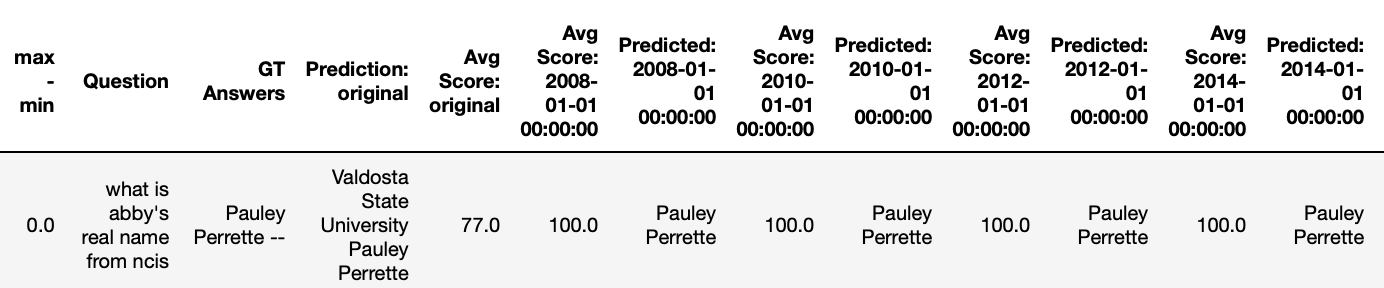
\includegraphics[width=5in]{timeless leven.png}
		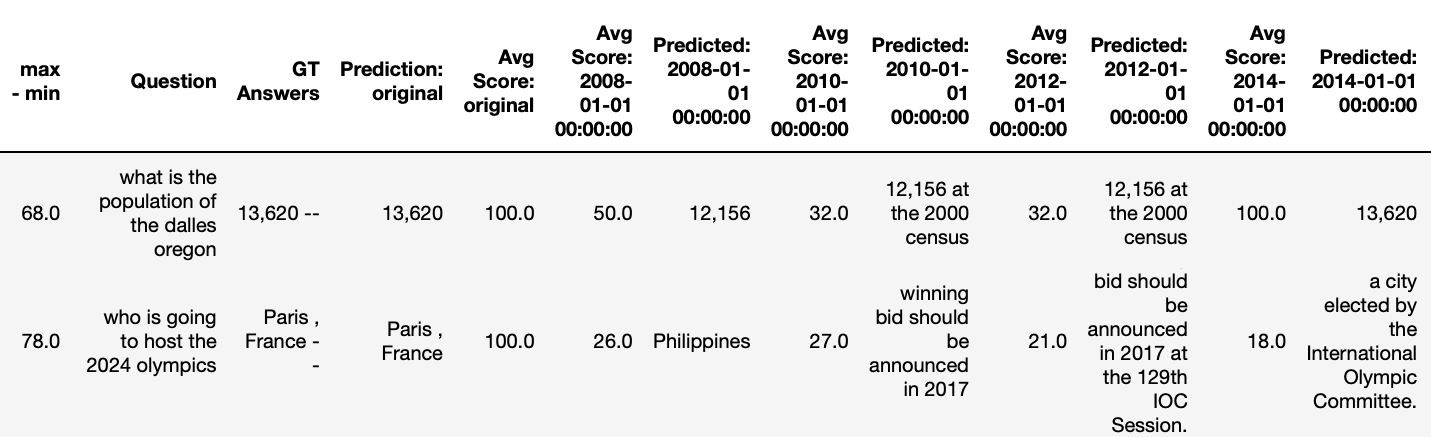
\includegraphics[width=5in]{timely leven.png}
		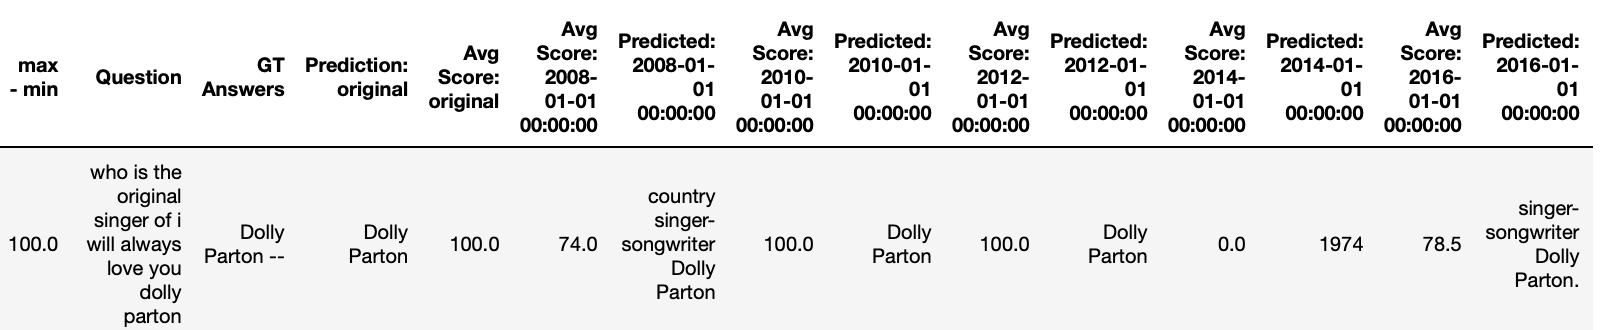
\includegraphics[width=5in]{leven false pos.png}
		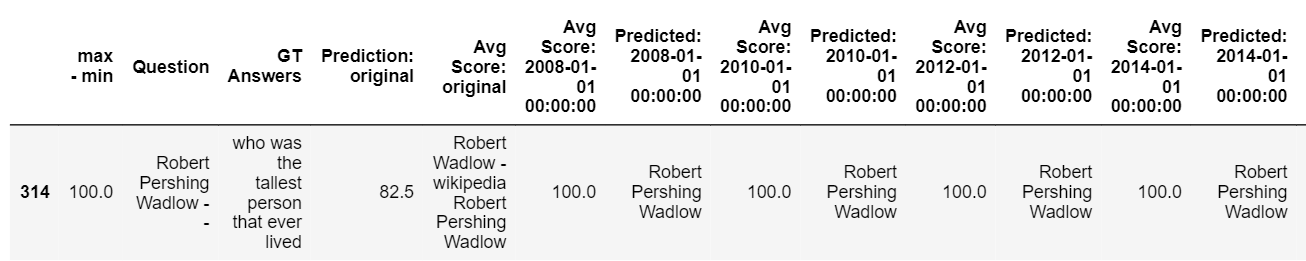
\includegraphics[width=5in]{leven_false_neg.PNG}
	\end{center}
	\caption{Levenshtein Examples (top is timeless, middle is timely, third is false positive, bottom is false negative).}
	\label{fig:levenshtein_examples}
\end{figure*}

After this initial filtering, our subset of 20,000 questions and answers was
reduced to 10,183 samples. Then, using the string Levenshtein distance, we
calculated the difference of each answer to the correct short answer provided in
the NQ dataset. Some questions had multiple correct short answers, in which case
we compared to the ground truth that had the closest match to the predicted
answer. Any samples which had an incorrect answer using the predicted answer
from the original HTML in the question were filtered out from our data. We
defined an incorrect answer as having a string comparison score of at least 70.
After removing these samples, we were left with a dataset of 3,408 samples to
work with.

\subsubsection{Answer Scoring}
We defined the string distance score using the functions in the {\tt fuzzywuzzy}
library. This was an implementation of the Levenshtein distance that included
two scores: token set score and token sort score. Token set score compared
across the entire strings, while for the token sort score, the order of the
tokens did not matter. We computed the average of both these scores for all the
answers outputted from BERT compared with the ground truth answer. Next, for
each question we computed the maximum string score and minimum string score and
subtracted the two, with the intuition that if the range was large, then the
answer would have changed a lot over the years.

Similarly, we also used BLEU scores to compare answers. In the implementation of
BLEU scores that we used, we were able to input multiple reference sentences and
obtain the best match with the test sentence. In addition, we could choose the
N-grams that the BLEU score used. Since we used short answers from the NQ
dataset and our predictions were only a few words long, we decided to use
unigrams and bigrams.

We computed four BLEU scores for each year’s predicted answer.
\begin{enumerate}
	\item Bigram BLEU: Bigram BLEU score based on the predicted answer and the
	      ground truth answer.
	\item Unigram BLEU: Unigram BLEU score based on the predicted answer and the
	      ground truth answer
	\item Previous years only Bigram BLEU: Bigram BLEU score between the predicted
	      answer and using all the answers from the years before it as the reference.
	\item Previous years only Unigram BLEU: Unigram BLEU score between the
	      predicted answer and using all the answers from the years before it as the
	      reference.
\end{enumerate}

The scores across the years were averaged to get four scores for each question.
The maximum of these scores was used to qualify timely and timeless questions.
Timely ones would have low maximum BLEU scores and timeless ones would have
higher ones.

\section{Results}
\label{results}
\begin{figure*}[ht]
	\begin{center}
		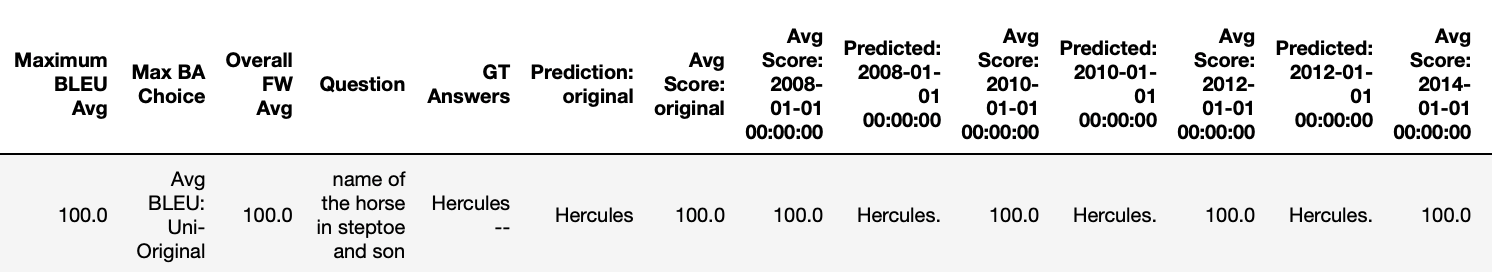
\includegraphics[width=5in]{timeless bleu.png}
		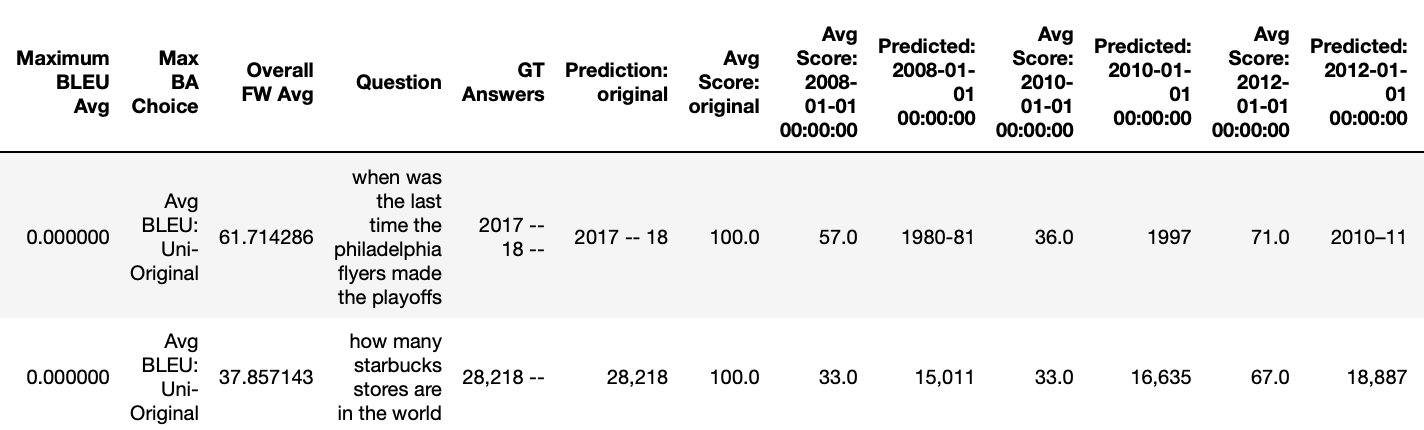
\includegraphics[width=5in]{timely bleu.png}
		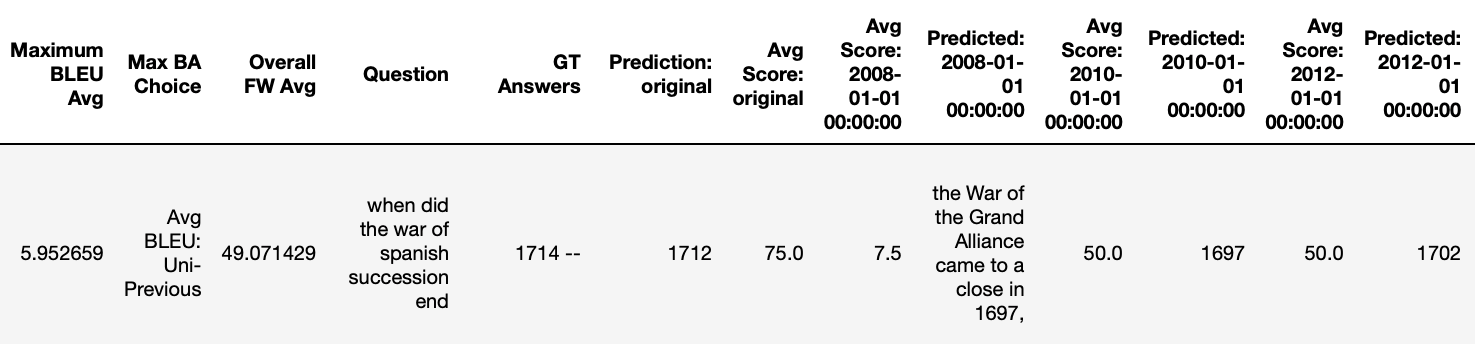
\includegraphics[width=5in]{bleu false pos.png}
	\end{center}
	\caption{BLEU Examples (top is timeless, middle is timely, bottom is false positive).}
	\label{fig:bleu_examples}
\end{figure*}

\subsection{Levenshtein Results}
\label{fuzzy results}

We first evaluated the answers using the aforementioned string distance score.
Generally, questions with a small difference between the maximum and minimum
Levenshtein distance were reliably timeless. Despite the rarity of timely
questions in our dataset, our approach was still somewhat effective at
identifying them. Many questions that had a larger Levenshtein range were found
to be timely.

Examples of correctly identified timeless and timely questions are shown in Fig.
\ref{fig:levenshtein_examples}. Depicted are timely questions, such as those
associated with changing populations or future events. We can note how the
model’s answer changes over time. While changes such as difference in population
are identified as expected, long, vague, or incorrect model outputs are still
present. Both these differences in actual answer and model performance
contribute to incorrect classification. Looking at the example timeless
question, we see the model output remains the same over time, so our Levenshtein
range is very small.

Despite its potential, we found that the model’s ability to detect timely
questions well was dependent on its ability to provide accurate answers.
Oftentimes, the model would output an unreasonable answer for a single year,
resulting in a higher Levenshtein distance between the ground truth. This caused
false positives, depicted in Fig. \ref{fig:levenshtein_examples}. In order to
tackle these issues, we explored methods to try and filter excessively long
model outputs, but decided to utilize the BLEU score as an alternative metric to
better capture semantic similarity.




\subsection{BLEU Results}
\label{bleu results}

Using BLEU score metrics, identifying timeless vs timely questions was more
successful. High BLEU scores corresponded to timeless questions and lower ones
were indicative as timely questions. Similar to Levenshtein, the highly
represented class of timeless questions were found reliably amongst those with
the highest maximum BLEU score. An example is seen in Fig.
\ref{fig:bleu_examples} where the answers are non--changing. Timely questions
found within the lowest scores showed changing answers and didn't have poor
model output present. While inconsistent answers may have had a confounding
effect on the Levenshtein approach, the BLEU score could ignore bad output and
decrease the prevalence of false positives. Additionally, in the cases of false
negatives, while there was poor model output present, there were also changes in
answers seen in Fig. \ref{fig:bleu_examples} where the year would change. These
were incorrect yet reasonable answers.

In general, the concentration of timely questions within the bottom 5 percent of
maximum average BLEU scores was much higher than that of its Levenshtein
counterpart. This was explained by BLEU score’s ability to be more robust to
outliers and its use of “distance” from previous answers, not just the dataset’s
ground truth answers. The latter difference allows for each year’s output to be
directly compared to one another; Levenshtein only compared outputs with the
ground truth. This allowed for a more intuitive approach to checking change over
time. In being able to use previous years’ answers as reference sentences to
test candidate answers against, a single year’s poor output does not impact any
average BLEU score. Since the wibbly output is often one of many reference
sentences, BLEU scores with previous--year reference sentences can calculate the
score using more accurate outputs. So although poor model output was still the
main reason for timeless questions amongst timely questions, the prevalence of
these was much lower when using BLEU. Despite one wobbly output, the BLEU score
could still remain high and accurately qualify a question as timeless.





\begin{figure}[t!]
	\begin{center}
		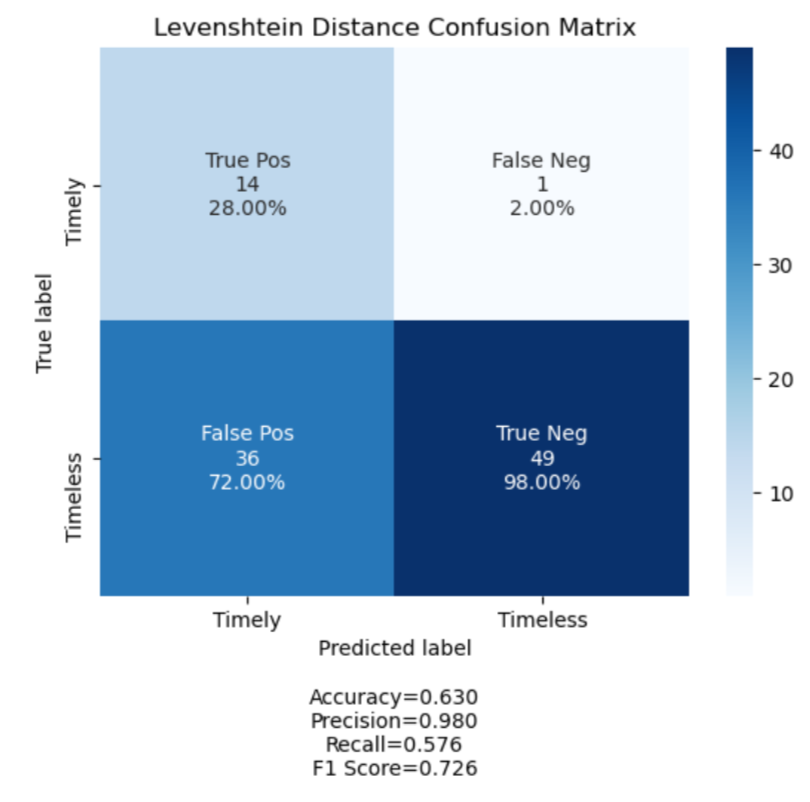
\includegraphics[scale=0.5]{leven.PNG}
	\end{center}
	\caption{Confusion Matrix for Levenshtein Approach}
	\label{fig:confusion_leven}
\end{figure}


\begin{figure}[t!]
	\begin{center}
		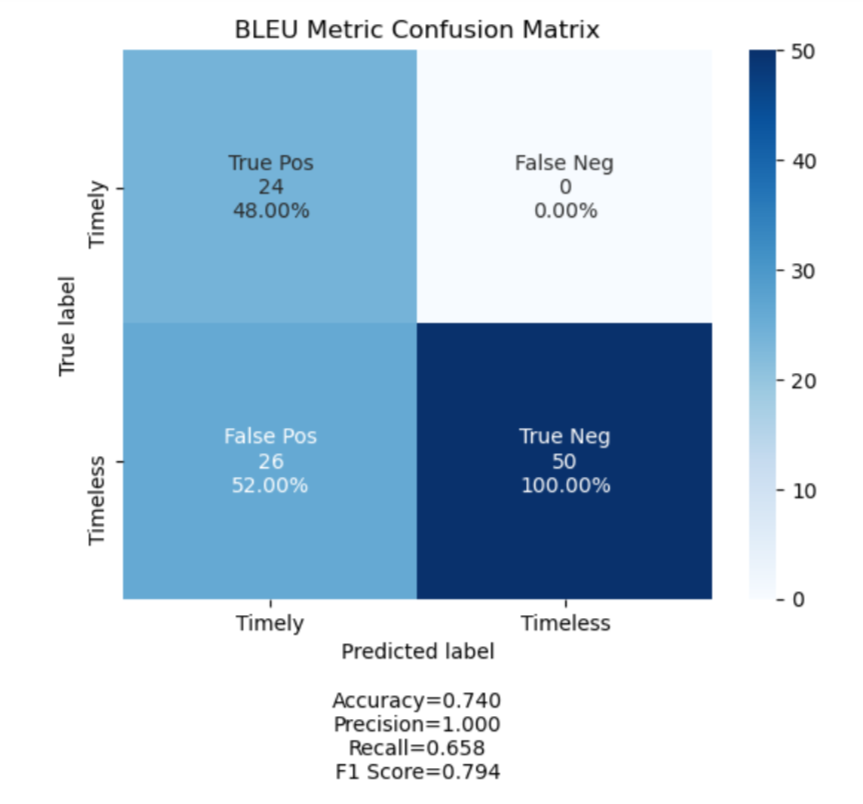
\includegraphics[scale=0.5]{bleu.PNG}
	\end{center}
	\caption{Confusion Matrix for BLEU Approach}
	\label{fig:confusion_bleu}
\end{figure}

\subsection{Quantitative Analysis}

To further investigate the efficacy of the two different metrics, we selected
two sets of fifty questions that were filtered as timeless and timely. We then
manually tallied the number of correctly classified questions for each set and
visualized the results via confusion matrices along with their respective
metrics in Fig. \ref{fig:confusion_leven} and Fig. \ref{fig:confusion_bleu}.
Generally, we can observe that using the BLEU metric as a filter substantially
reduces the number of timeless questions falsely predicted as timely, thereby
increasing the accuracy and recall compared to the Levenshtein approach. Since
we expected roughly 10\% of questions to be timely, this means that for both of
our models, we were able to detect timeliness better than chance. However, the
proportion of questions with a low BLEU score is much smaller than the
proportion of questions with a high Levenshtein range. This suggests that our
current methodology may result in a higher number of false negatives with BLEU
approach.


\section{Limitations}
While the BLEU score results are promising, there are some significant
limitations with this methodology. The BLEU score approach filters out a large
number of questions, giving a very high false negative rate. As for the
Levenshtein methodology, we found that our timely detection rate was tightly
linked with how well our model behaved. In general, we would expect that our
model would have performed significantly better had it been trained on the NQ
dataset beforehand. This would give our string metrics much more reliable data
and improve the quality of our results. In addition, we had to filter out the
majority of the dataset before even running our string comparisons largely due
to issues with Wikimedia's API. We ended up filtering roughly 10,000 out of the
20,000 total questions because of these issues. An additional 7,000 were
filtered from poor model performance.

Even with a perfect pre--trained model, we still run into some key limitations
with our methodology. The first is that we assume that the answer to any
question in the dataset can be found within the first 25 paragraphs. An analysis
done by Google for the NQ dataset found that roughly 70\% of questions can be
found in a paragraph tag, but that leaves roughly 30\% of questions that have
answers in a table (which we do not add into our model inputs) \cite{nqdataset}.
Finally, as noted in the Results section, if a question’s answer has not changed
in the past 10 years, then our methodology will produce a false negative.

% Acknowledgements should only appear in the accepted version.

\section{Future Work}
With a longer project timeline, we would have liked to retrain a BERT model
ourselves on the NQ dataset to get a more accurate model. In addition, once we
have a more accurate set of timely and timeless questions, we would train a
language model to classify questions based on their timeliness.

\section{Contributions}
\subsection{Vatsal Agarwal}
Vatsal helped with dataset processing and analysis, as well as the presentation
and paper work.
\subsection{Pauline Comising}
Pauline ran the Google Trends baseline, helped with Wikimedia API integration,
implemented BLEU score calculations, and helped with presentation and paper
writing.
\subsection{Harish Kumar}
Harish ran the Google Trends baseline. He also helped with presentation and
paper writing.
\subsection{Madhava Paliyam}
Madhava ran the BERT-SQUAD model on the train and development datasets. He
implemented the comparisons using the {\tt fuzzywuzzy} package. He also helped
with the analysis.

\subsection{Nikhil Pateel}
Nikhil worked on the Google Trends baseline, Wikimedia API integration, as well
as presentation and paper preparation.


\section*{Acknowledgements}

We would like to thank Professors Jordan Boyd-Graber and Phillip Resnik for
guidance on our project, as well as UMD for providing computational resources to
make this project possible.


% In the unusual situation where you want a paper to appear in the
% references without citing it in the main text, use \nocite
%\nocite{radev2002using}
%\nocite{breck2000another}
%\nocite{jia2018tequila}
%\nocite{nqdataset}
%\nocite{squaddataset}
%\nocite{nltk}
\bibliography{main}
\bibliographystyle{icml2021}




\end{document}


% This document was modified from the file originally made available by
% Pat Langley and Andrea Danyluk for ICML-2K. This version was created
% by Iain Murray in 2018, and modified by Alexandre Bouchard in
% 2019 and 2021. Previous contributors include Dan Roy, Lise Getoor and Tobias
% Scheffer, which was slightly modified from the 2010 version by
% Thorsten Joachims & Johannes Fuernkranz, slightly modified from the
% 2009 version by Kiri Wagstaff and Sam Roweis's 2008 version, which is
% slightly modified from Prasad Tadepalli's 2007 version which is a
% lightly changed version of the previous year's version by Andrew
% Moore, which was in turn edited from those of Kristian Kersting and
% Codrina Lauth. Alex Smola contributed to the algorithmic style files.
